\begin{figure}[!t]
\begin{center}
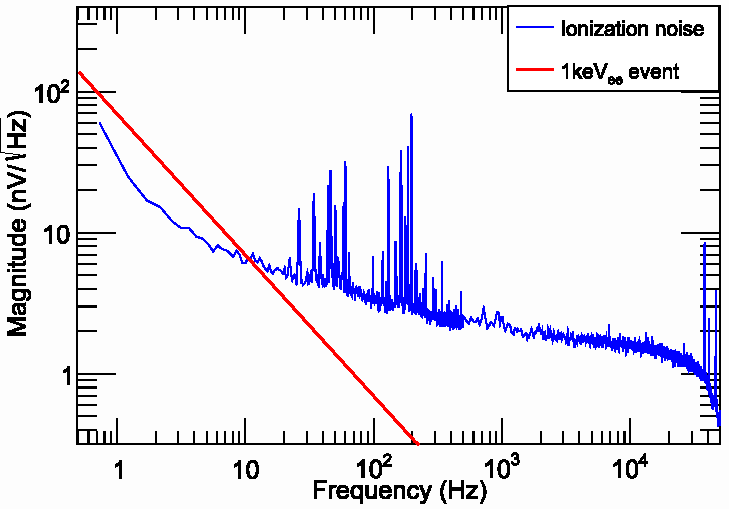
\includegraphics[width=\textwidth]{./fig/Rauschen/EDWIIIPerformance.pdf}
\vspace{-0.5cm}
\caption{Leistungsdichtespektren der EDELWEISS-III Ausleseelektronik \cite{EDWIII}.}
\label{fig:EDWIII}
\end{center}
\end{figure}

Eine Aussage über die Energieauflösung ist erst möglich wenn sowohl das Rauschen als auch die Form des Signals bekannt sind.
Für die Bestimmung der Energieauflösung ist es also notwendig einen Beispielsignal wie wir es erwarten würden zu bestimmen.
Wie in den Kapiteln \ref{sec:Entstehung} und \ref{sec:Elektronik} gezeigt erzeugt ein Event welches die Energie $E$ deponiert eine bestimmte Zahl Elektron-Loch-Paare $N_{eh}$ abhängig von einer Materialspezifischen mittleren Energie zur Erzeugung eines Elektron-Loch-Paars $\epsilon$.
Für den Strom der durch ein solches Event in der Elektronik induziert wird ergibt sich somit
\begin{equation}
I_{sig}(t) = e\frac{E}{\epsilon}(a-b)\delta (t).
\end{equation}
Durch die transformation in den Frequenzraum und Multiplikation mit der Eingangsimpedanz erhalten wir das Spektrum des Signals
\begin{equation}
s(f) = e\frac{E}{\epsilon}(a-b)\frac{1}{2\pi f C_{ges}}.
\end{equation}
Die Bestimmung der Energieauflößung mittels der Optimal Filtering Methode ist gegeben durch
\begin{equation}
\sigma^2_E = \left(\sum_{f_{min}}^{f_{max}}\frac{|s(f)|^2}{J_{ss}(f)}\Delta f\right)^{-1}
\label{eq:OptFilt}
\end{equation}
$f_{max}$ - $f_{min}$ ist die Bandbreite, $J_{ss}$ die Leistungsspektrumdichte für $f>0$ und $\Delta f$ der Abstand zwischen den gemessenen Frequenzen.
Aus dieser Gleichung lässt sich erkennen, dass die Verstärkung keinen Einfluss auf die Auflösung hat, da sowohl das signal $s(f)$ als auch das Rauschen $J_{ss}$ gleichermaßen verstärkt werden.
Die Verstärkung muss nur groß genug sein sodass das Rauschen der Nachfolgenden Elektronik keine Rolle spielt.
Auf diese Weise wurde für das in Abbildung \ref{fig:54ROpen} gezeigte Rauschen eine Energieauflöung von $\boldsymbol{\sigma_E = \frac{1}{a-b}\cdot 1.31\,\mathrm{keV}}$ berechnet unter der Annahme einer Detektorkapazität von $\SI{150}{\pico\farad}$.
Man sieht, dass die Auflösung proportional zum Prozentsatz des von den Ladungsträgern durchlaufenen Potentials $(a-b)$ ist.

In Abbildung \ref{fig:EDWIII} ist das Leistungsdichtespektrum der EDELWEISS-III Ausleseelektronik dargestellt zusammen mit einem $\SI{1}{\kilo\electronvolt}$ Beispielsignal.
Damit wurde eine Energieauflösung von $\SI{500}{\electronvolt}$ erreicht\cite{EDWIII} unter Verwendung eines $\SI{150}{\pico\farad}$ Detektor mit zusätzlich $\SI{100}{\pico\farad}$ Kapazität durch die Kabel und $\SI{50}{\pico\farad}$ Eingangskapazität des JFET.
Die beste von Axel Gullasch erreichte Energieauflößung mit der gleichen Elektronik ist $\SI{2.11}{\kilo\electronvolt}$ \cite{Gullasch2015}.
%TODO Detektorkapazität nicht bestimmt Gullasch
Mit CRNS/LPN HEMTs ist eine Energieauflösung von $\SI{91}{\electronvolt}$ mit einem $\SI{150}{\pico\farad}$ CDMS-Detektor gelungen \cite{Phipps2016}.

